\section{Question 3: Joint vs.\ Individual Taxation --- Labor Supply}

\subsection*{Setup}

We compare labor supply under two tax systems. Both members start with $K_{1,0} = 2$ and $K_{2,0} = 0$, meaning member 1 has some initial human capital while member 2 starts with none.

Under \textbf{joint taxation}, the household is taxed on combined income:
%
\begin{equation}
    T_{\text{joint}}(Y_1, Y_2) = \left(1 - \lambda^{\text{joint}} (Y_1 + Y_2)^{-\tau^{\text{joint}}}\right) \cdot (Y_1 + Y_2)
\end{equation}
%
with $\lambda^{\text{joint}} = 2.28$ and $\tau^{\text{joint}} = 0.0861765$.

Under \textbf{individual taxation}, each member is taxed on their own income:
%
\begin{equation}
    T_{\text{indiv}}(Y_1, Y_2) = \left(1 - \lambda^{\text{indiv}} Y_1^{-\tau^{\text{indiv}}}\right) Y_1 + \left(1 - \lambda^{\text{indiv}} Y_2^{-\tau^{\text{indiv}}}\right) Y_2
\end{equation}
%
with $\lambda^{\text{indiv}} = 1.75$ and $\tau^{\text{indiv}} = 0.0646416$.

\subsection*{Results}

We solve and simulate both models and plot the average hours and income of each member over the life cycle.

\begin{figure}[H]
    \centering
    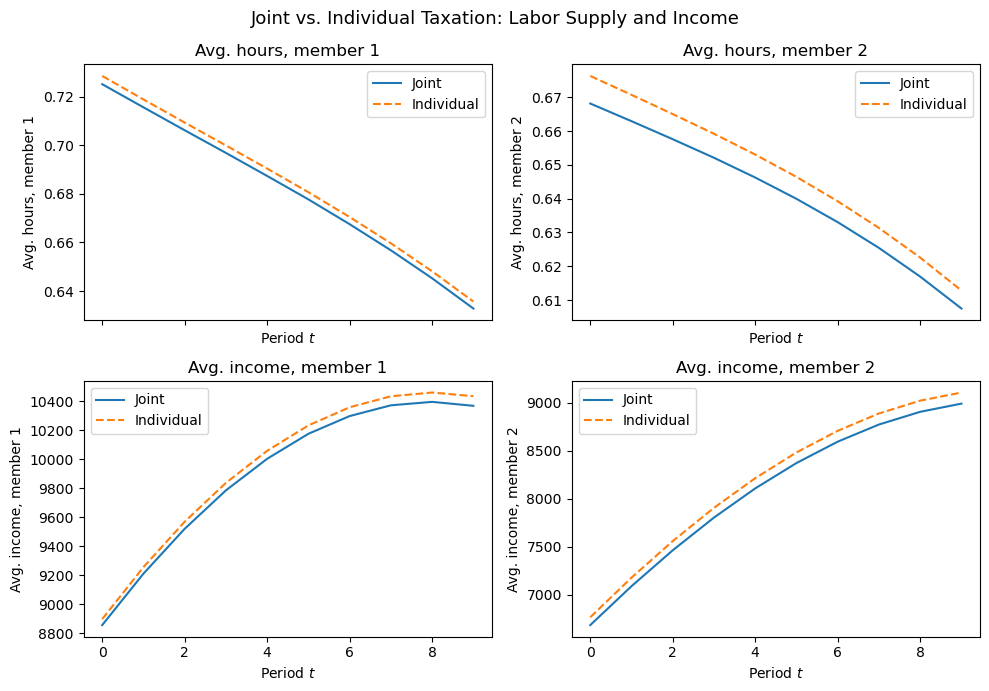
\includegraphics[width=0.7\linewidth]{Billeder/plot 4 ny.png}
    \caption{Average hours and income per period under joint vs.\ individual taxation ($K_{1,0}=2$, $K_{2,0}=0$); member 2 works more under individual taxation.}
    \label{fig:placeholder}
\end{figure}

\subsection*{Discussion}

The key difference comes from how the tax systems treat the secondary earner. Under joint taxation, the lower-earning member (member 2, who starts with $K_{2,0}=0$) faces a higher marginal tax rate because their income is added on top of member 1's income. This discourages member 2 from working. When we switch to individual taxation, member 2 is taxed on their own (lower) income separately, which means a lower marginal tax rate and therefore a stronger incentive to supply labor. As a result, member 2 works more under individual taxation, while the effect on member 1 is smaller.

This static incentive is amplified dynamically. Because human capital accumulates as $K_{j,t+1} = (1-\delta)K_{j,t} + h_{j,t}$ and wages rise in $K$, the extra hours member~2 supplies early under individual taxation build up human capital, which raises later wages and feeds back into still higher labor supply later in life. The gap between the regimes therefore widens over the life cycle rather than staying constant --- which is precisely why a dynamic, rather than static, model is needed to capture the reform.
